%! Author = Marjan
%! Date = 02/02/2025
% Preamble
\documentclass[a4paper, 11pt]{book}

% Packages
\usepackage{amsmath}    % For math symbols and equations
\usepackage{graphicx}   % For including graphics
\usepackage{geometry}   % For adjusting page layout
\usepackage{fancyhdr}   % For custom headers/footers
\usepackage{hyperref}   % For hyperlinks
\usepackage{listings}   % For code listing
\usepackage{lipsum}     % For placeholder text (to test layout)
\usepackage{helvet}
\usepackage{arydshln}
\usepackage{wasysym} % Helvetica as a sans-serif font alternative
\renewcommand{\rmdefault}{phv} % Set the default font family to Helvetica

% Set page margins (A4 paper)
\geometry{top=1in, bottom=1in, left=1in, right=1in}

% Set up the header
\pagestyle{fancy}
\fancyhf{}
\fancyhead[L]{System Design Notes}
\fancyhead[C]{Your Name}
\fancyhead[R]{\thepage}

% Document
\begin{document}

% Title Page
    \begin{titlepage}
        \centering
        \vspace*{2in}
        \Huge \textbf{System Design Notes}
        \vfill
        \Large Your Name
        \vfill
        \Large Date: \today
    \end{titlepage}

    \newpage

    \tableofcontents
    \newpage


    \chapter{Introduction}


    \section{Goals of this document}
    The goal of this document is to collate information that I think is useful in the area of software architecture.


    \section{OSI Model}
    Very useful when operating on different levels of abstraction in a system

    \paragraph{Level 1} - Physical

    \paragraph{Level 2} - Data link

    \paragraph{Level 3} - Network

    \paragraph{Level 4} - Transport

    \paragraph{Level 5} - Session

    \paragraph{Level 6} - Presentation

    \paragraph{Level 7} - Application


    \section{C4 Model}
    Very useful for handling different levels of abstraction

    \paragraph{Motivations: Why should I care}
    Drivers - Performance, Scalability, Fault Tolerance.
    How to measure.....latency, throughput, cost
    Consider SLA,SLO and SLI.
    Easier to code more complex stuff......


    \chapter{Gathering requirements}
    Asking is a user is not practice.
    A better and more methodical way of gethering requires ments of the desired system is through use cases and user flows.
    A use cases are a particular scenario/ situation in whcih the system is used to achieve a userss goal.
    A user flow is a more detailed step by step graphical representation of a use case.


    \section{Gathering functional requriements}
    In a formal way.
    First we need to identify all the actors or users in out system otherwise relevant usecases may not be caught.
    Second step is to describe all the possible use cases or sceanarios in which an actor can use our system.
    Finally the third step is to take each use case and expand it through a flow of events or interactions between the actor and the system.
    In each interaction we cature the action and take a note of the data that flows with it to and from the system.

    Multiple ways to represent this, one way is a sequence diagram which is a part of UML. Standard for viaualising system design.


    \section{Non functional requirements}
    These requirements have an effect on the software achitecture.


    \section{Why redesign}
    System is functionally correct but speed, scalabilty, maintence or security is too hard for reasons like number of users or data volume.
    System is functionally the same after redesign.
    Right achitexture from the start is important
    Quality measures are used to measure how well the system performs and correlate with the architecture.
    Quality attributes have to be measurable and testable and this must be consistent.

    Something to note is that no single architecture can provide all the quality attributes. Certain attributes contradict each other.
    Some combinations are hard/ impoissble to achieve. Tradeoffs are needed.

    Third important consideration of the system is feasiblilty of the quality attributes.
    Architect needs to ensure that the system is deliverable and what the client is asking for.
    Client could actually ask for something that is not technical or not technically possible.
    I.e expesive or not feasible. An example could be unrealistic latency expectations.
    Before approving a requirement, conslulting with a domain expert to ensure that the requirement can actually be delivered.

%    Three important quality attributes when desigining a system
    \begin{list}
        \item Testability and measurablility
        \item Make tradeoffs between quality attributes over others
        \item Feasibility of quality attributes
    \end{list}

    \section{System constraints}
    Once functional requirements are defined, system function is known there are usually multiple ways to achieve the desired system
    Quality attributes will lead to tradeoffs and this is normal.
    System constraints are refered to as \quote{pillars} of an architecture.
    System constraints provide a starting point since the are usually non-negotiable and the rest of the system has to be designed around it.

    Three types

    \begin{list}
        \item Technical - Being locked to hardware, cloud vendors etc, must be on prem, etc.
        \item Legal - Geography, different rules in different countries where the system resides.
        \item Business - Limited budgest, strict deadlines.
    \end{list}

    Once constraints are identified consider non negotiable constraitns and self-imposed constraints that can be removed.
    Once a set of constriants have been agreed it is hard to move away from them.
    If further in the project timeline it is found that some of those constraints were not really constraints, then the architecture will not make sense in the future.
    Another consideration is that when certain constraints are accepted, enough space needs to be left in the architecture to move away from those constraints in the future.
    Need to avoid tight coupling with certain components or constraints to allow for change otherwise whole system could be rearchitected.

    \section{Gathering System Requirements}

    \paragraph{Requirements} - Description of what we needs to be built.
    Very different when approached from a system level.
    Higher scope allows for freedom of tools and also requries a higher level of abstraction.
    Requirements are often not from an engineer or even someone technical.
    Requirements are only part of the solution.
    Client only knows the problem they need solved.
    Clarifying questions are required.

    \paragraph{Importance} - Simply build something and then fix it, wrong requirements etc, easy to fix?
    Large scale systems (i.e at this level) are big projects that cannot be changed easily.
    Many engineers invovled and many hours.
    Hardware and Software costs.
    Contracts and financial obligations.
    Reputation and brand


    \section{Type of Requirements AKA Architectural Drivers}

    \paragraph{}
    Features of the System - Functional Requirements - Describe the system behaviour i.e what the system must do - Tied to the object of the system
    This doesn't determine the architecture

    \paragraph{}
    Quality Attributes - Non-functional requirements
    System properties - Scalability, Availability, Reliability, Security, Performance etc
    This does dictate the architecture

    \paragraph{}
    System Constraints - Limitations and boundaries
    Examples - Time Constraints and Deadlines, Financial Constraints, Staffing Constraints


    \chapter{Quality attributes in large scale systems}


    \section{Performance}
Some performance metrics
    Response time - Tiem between client sending a request and recieve a response
    Two parts, the processing time with code and databases applying business logic.
    And the \quote{waiting} time. The duration of time that the request or response inacitvely spends in the system.
    This time is usually spend in transit in the physical network or in software queues waiting to be handled or reach its destination.
    Waiting time is also known as latency.

    Response time can also be called end to end latency and is an importnat metric.

    Another important metric is throughput, which is the amount of data a system can process in a given interval of time.
    The more per unit of time the higher the throughput.

    \subsection{Measuring}
    Consider the end to end response time.
    COnsider the distribution of response times and set a measure around it. Use a histogram, chart etc, statistics etc.
    Especialy consider tail latency, the resposnes that take the most time in comparison to the rest of the values.
    This tail latency needs to be as short as possible.
    Another consideration is the performance degradation point and how fast or steep the degradation is.
    This is the point in the performance graph where the performance is starting to get significantly worse as the load increases.
    Usually this means a resource is fully utilised, could be hardware resource etc or a software queue.

    \section{Scalability}


    \section{Availability}


    \section{Fault tolerance}


    \section{SLA. SLO, SLI}


    \chapter{API Design}


    \section{Relevance}


    \section{RPC}
    Does gRPC fit in here?


    \section{REST}


    \section{GraphQL}


    \chapter{Large Scale Systems Architectural Building Blocks}


    \section{DNS, Load Balancing}


    \section{Message Brokers}
    Kafka.....


    \section{API Gateways}


    \section{CDN Solutions and cloud}


    \chapter{Data storage at less trivial scale}


    \section{Relational Databases and ACID Transactions}


    \section{Non-Relational Databases}


    \section{Techniques to improve performance, availability and scalbilty of databases}


    \section{CAP Theorem}


    \section{Scalable unstructured data storage}


    \chapter{High-Level System Design}

    \paragraph{Software Architecture Patterns} - General repeatable solutions to commonly occurring system design problems.
    Versus design patterns which are just about organising code within a single application.
    Software architectural patterns are \quote{blueprints} for solutions that involve multiple software components.
    The purpose is to avoid repeating mistakes and antipatterns for large scale systems.

    \paragraph{Business incentives for this approach} - One - Save time and resources for devs and the organisation
    when building a solution on a similar scale.
    Use already tested development practices rather than reinvent the wheel,
    something completely new can potentially take up a lot of resources.

    \paragraph
    Two - Using an existing architecture avoids the \textit{big ball of mud}.
    The lack of structure on the system.
    In this scenario every service talks to every other service, services are tightly coupled, information is global or duplicated
    and there is no clear scope or responsibility for any of the components.

    \paragraph
    This situation can happen due to rapid growth of the company or a lack of architecture in general.

    \paragraph
    In this situation a system can be hard to develop, maintain and scale which in turn can lead to the failure of business objectives.

    \paragraph
    Third motivation - Other developers and architects can continue working on the system and can easily carry on and stick to the same architecture.
    Everyone will know the pattern that is being followed and understand what should and should not be done when adding to the system.

    \paragraph
    These are just guidelines.
    Architecture is best defined per use case / unique situation.
    As systems evolve certain patterns that were appropriate to the system in the past may not make sense anymore.
    This is normal.
    At this point some restructuring would need to be done and a migration to a different architecture pattern should be considered.

    \paragraph
    Motivations for patterns - many companies have already been through these migrations before so best practices can be adopted to make those migrations quickly and safely.

    \subsection{N/Multi-Tier Architecture}

    \paragraph{Intro}
    Organise the system into multiple physical and logical tiers.
    Logical separation limits the scope of responsibility.
    Physical tier allows each tier to be deployed, upgraded, scaled separately by different teams.

    \paragraph{}
    Note: Multi-tier and Multilayer are two different concepts.
    Multi layered architecture usually refers to the internal sepration inside a single application into multiple logical layers or modules.
    Even if the application is logically seprated into multiple layers at runtime it will run as a single unit and will be considered a single tier.

    Multi-tier architecture - applications on each tier run physically run on different infrastructure.

    \paragraph{}
    Benefits of logical and physical separation-Allows us to develop update and scale each tier independently.
    Restrictions in this architectural pattern.

    \paragraph{}
    First restriction is that each pair of applications that belong to adjacent tiers communicate with each other using the Client-server model.
    REST etc.
    Second restriction - discourages communication that skips through tiers.
    This keeps the tiers loosely coupled with each other allowing for easy changes between tiers withouth effecting the entire system.

    \paragraph{Three tier - Common variation}
    \hrule
    Top level contains UI aka presentation tier.
    Display information and take user input through a GUI.
    No business logic normally, this tier usually runs in the client browser. I.e JavaScript etc.
    The code here should be assumed to be visibile and accesible to the user. Bad place for business logic doing so is considered an anti-pattern.
    \hrule
    Application Tier / Business Tier/ Logic Tier.
    Provides the logic gathered from functional requirements.
    Responsible for processing the presentation tier and applying the relevant business logic to it.
    \hrule
    Data tier, this tier is responsible for storage and persistence of user and business-specific data.
    Tier may include files on a local file system or a database.

    \paragraph{Why so popular?}
    Fits a large number of use cases.
    A lot of web based services fit this model, shops, news sites etc etc.
    Very easy to scale horizontally to take large traffic volumes and handle more data.

    \paragraph{How does it scale}
    The presentation tier runs on a users device so it scales by itself....get a better phone / computer etc.
    \hrule
    Application Tier - if it is kept stateless, application instances can be kept behind a load balancer and run as many instances as we need.
    \hrule
    Database / Persistence tier - can be easily scaled if a well established distributed data base is used. DB scala - replication, partioning, sharding etc.

    \hrule
    This architectural pattern is very easy to maintain and develop because all the logic is concentrated in one place; the application tier.
    Most backend development should happen in the application tier.

    No need to worry about integration of different code bases, services or projects.

    \paragraph{Weaknesses of this pattern}

    Major drawback, the monolithic structure of the logic tier. Business logic should not be placed in the presentation or data tier.
    Issue is all the business logic is concentrated in a single user code base that runs as a single runtime unit.
    The implications of this, each instance of the application becomes too CPU intensive and will consume too much memory.
    This makes the appilication too slow and less responsive.
    This can especially be a problem with memory managed/ GC language like Java and C\# (maybe add go to this list)
    As a result applications can have longer and more frequent garbage collections.
    This can lead to requring an upgrade of the computer the application is running on.
    Vertical scaling is both expensive and limited.

    \paragraph{}
    The second impact of the monolithic application tier is low development velocity.
    More complex code base makes it harder to develop maintian and reason about the code.
    Hiring more developers to solve this problem will not solve the problem/ add value.
    Why?
    Because more concurrent developers will simply cause more merge conflicts and higher overhead.

    \paragraph{}
    Mitigation: Could split the code into modules based on logic.
    The modules will be somewhat tightly coupled since we can release new versions of those modules only when the applications has been upgraded.
    I.e the organisational scalability of the Three-tier architecture is limited.
    Best when the code base is relatively small and not that complicated and will be maintained by a small team of developers.

    \paragraph{Examples}
    Early startups, well established companies that fit the criteria above.

    \paragraph{Variations of the Multi-Tier Architecture}
    One Tier
    Two tier - Business logic and presentation tier is combined.
    Think mobile or desktop application.
    Data tier handles persistence.

    \hrule
    More complexity - four tier.
    Between the presentation tier and the business logic tier.
    Between this tier functionality that does not belong in either can be seprated.
    Could introduce API Gateway tier that handles security,caching, data formats etc when communicating between different systems.

    \hrule
    More than four tiers is rare since they do not usually provide more value and simply adds more performance overhead.
    The source of this overhead comes from not being able to bypass tiers so as to avoid tight coupling.
    Every request would have to pass through multiple services which can increase response time/latency.
    Rarely a request would have to do so much travelling.

    \subsection{Microservices}

    \paragraph{Motivations}
    The size and complexity of the code base has grown, troubleshooting and adding new features.
    building, testing and even loading code into the IDE is now cumbersome.
    Organizationally, we now have problems.
    More developers leads to more merge conflicts, longer, larger and less productive meetings.
    At this point microservices should be considered.

    \paragraph{Microservices}
    Organises business logic as collection of loosely coupled and independently deployed services.
    Each service is owned by a small team and has a narrow scope of responsibility.

    \paragraph{Advantages}
    Codebases are now \textit{smaller} .
    Development is a lot easier and faster along with deployment and testing.
    Simply because there are less things.
    Code is easier to reason about and features can be added faster.
    New developers can become productive faster.
    Regarding performance and scalability, each microservice becomes less CPU intensive and takes less memory and can now run much more smoothly on commodity hardware (cloud).
    Can scala horizontally by adding more instances of low-end computers.
    Organizationally, the advantages are each service can be independently developed, maintained and deployed by a separate small team.
    This can lead to high throughput from the organisation as a whole.
    Each team can be autonomous with regard to tech stack, release schedule or process they want to follow.
    Better security in the form of fault isolation, i.e if one service starts crashing its easier to isolate and solve.

    \paragraph{Note} - Organisations can move to this architecture too quickly, without considering two factors.
    First - theoretically can achieve all those benefits from migrating to microservices, but they don't just happen and this can easily end up as a big ball of mud
    Second - microservices come with a fair amount of overhead and challenges.

    \paragraph{Pre microservices}
    To achieve full organisational decoupling so that each team can operate independently, services need to be logically seprated in way that every changed in the system can happen only in one service.
    This is to avoid involving multiple teams.
    If a change requires multiple teams then not much is gained from this migration.

    \paragraph{Microservices best practices}
    Single responsibility principle - each microservice needs to be responsible for one business cpabilyt domain resource or action.
    Monolithic API gateway can be decomposed into multiple microservices, making them more lightweight and specialised.
    Second practice is to make sure there is no coupling between different services, and this can be achieved by having a differnt database for each service.
    Note: If two services share a database then every single schema or document structure change will result in complext coordination between teams.
    If each service has its own DB then it just becomes an implementation detail that can be easily updated or replaced completly without implacting the rest of the system.

    \paragraph{Splitting the data}
    When splitting a monolithic database the data has to be split in a way that each microservice can be completely independent and fully capable of doing its work while minimising the need to call other services.
    Data duplication is expected and is normal in this scenario.
    Duplication is a tradeoff here and an overhead of using this architecture.

    Following best practices will help achieve a positive outcome when moving to microservices.

    \paragraph{Practical note}
    Microservices brings in additional complexity and overhead.
    This only brings business value when the system reaches a certain size and the organisation is of a certain scale.
    Start with a monolith approach first.
    When that is no longer working for the use case, then move to micro services.

    \paragraph{Conclusion}

    The benefits of microservices architecture.
    Higher organisational and operation scalability, better performance, faster development, better security.
    Best practices are required to realise these advantages and are only really applicable to systems and organisations of a certain size.

    \subsection{Event-Driven Architecture}

    \paragraph{Motivation}
    If microservice A want to communicate with Microservice B, then not only does it require awareness of service B, it also needs to know how to call what API microservice B provides and how to call it at run time.
    Also microservice A has to call microservice B synchronously and wait for its response (No always async etc????).
    Microservice A has a dependency on microservice B.

    \paragraph
    In an event driven architecture, instead of direct messages that issue commands or request that ask for data, we have only events.
    An event is an immutable statement of a fact or a change.
    In an Event-Driven architecture we have three components.
    Sending side - We have event emitters, which are also referred to as producers.
    Receiving side - We have event consumers
    And inbetween we have the event channel (a message broker), Kafka?

    \paragraph{Advantages}
    When we use the Event-Driven Architecture style with microservices we can get a lot of benefits.
    Now the dependency between Microservice A and B is removed.
    Microservice A doesn't need to know anything about the existence of microservice B
    And once microservice A produces the event, it doesn't need to wait for any response from any consumer.
    Because services don't need to know about each other's existence or API and all the messages are exchanged completely asynchronously, we can decouple microservices more effectively.
    This results in higher scalability.
    More services or integrations can be added to to the system without making any changes.
    Horizontal and organisational scalability is achieved via EDA.
    This architecture also allows us to analyse streams of data, detect patterns and act up on them in real time.

    \paragraph{Further advantages}
    When all events that occur in a system are stored in a message broker, in addition to data analysis an very powerful architecture pattern can be implemented.
    This is called event sourcing.
    By using event sourcing events can be replayed to identify the current state of a system rather than saving the state in a database.
    Because events are immutable we never modifying them.
    We simply append new events to the log as they come.
    Using event sourcing we can store events for as long as we want.
    Querying can be made faster by adding snapshot events.

    \paragraph{CQRS}
    Another architectural pattern that can be implemented as a result of EDA
    Command query responsibilty segregation.
    This solves two problems.

    First problem is optimizing a database that has a high read and update operations.
    In this scenario concurrent operations to the same record or tables contend with each other making the system slow.
    Additionally if we use a distributed database, generally we can optimise it for one type of operation at the expense of teh other.
    (Cap theorem?)
    Ad-hoc solution - We can optimise one operation at the expense of the other when an application is read/write heavy.
    However when the both operations are equally important we have a problem.
    CQRS achitectural pattern allows us to separate Update and Read operations into separate databases, sitting behind seprate services.
    In this case service A would take all the update operationss and perform them in their own database, where it optimially stores the data for such updates.
    Additionally every time an update operation is performed if publishes an event into a message broker.
    Meanwhile service B will subscribe to those update events and applies those changes in its own read otimised database and now all read operations will go to service B.
    Both update and read operations can go to separate services without any contention/interference.

    Further, the data can be optimised for each type of operation.


    The second problem that CQRS helps solve is joining multiple tables that are located in seprate databases that belong to two differnt microservices.
    Prior to monoliths all data was in one table. If that was a relational databse all the records could be joined and then analysed.
    Post microservices, this is not the case assuming that best practice has been followed. Joins are harder now.
    Requests need to be sent to each service separately which is slower.
    This data needs to be combined programattically becasue now we potentially have differnt types of databases.
    Some of these databases may not even be relational.


    CQRS solves this problem. Every time there is a change of data in a services database, those services would publish those changes as an event to which other services subscribe to.
    The other service will store what is called a materialized view of the joined read-to-query data from both service A and service B in its own read-only database.
    Whenever we need to get a join view we can just send a request to the joining service rather than send a request to two services.

    \paragraph{summary of EDA}
    When combined with microservices this allows for decoupling of services potentially allowing for horizontal and organiszation scalability.
    Event driven architecture allows us to analyse and respond to large streams of data in real time.

    \paragraph{Pattern within EDA}
    Event sourcing - allows for the auditing and storage of the current state of a business entity by only appending events and replaying them when needed.
    CQRS - Allows for database optimisation for both updates and reads by splitting the operations into separate services.
    This allows for the efficient joining of data from separate services.

    \chapter{Microservices}

Dedicate this part to microservices
%   Consider combining this with the other microservices section


    \chapter{Microservices in depth}

    \paragraph{Note} EDA and Microservices aren't a requirement for each other but they are commonly used together to achieve greater decopuling.
    Issues to address with Microservices, organisational scaling and technical problems relating to scaling.
    Refactoring is harder and application becomes less stable, small issues can jeopardise the whole system.
    Solution, organise business logic as loosely coupled deployable independently deployable services.
    Each service is owned by a small team and has narrow scope of responsibility.
    Now we have organisational scalability, building is faster, less burden on the developer, each binary is smaller in size.
    Testing and reasoning is easier, onboarding is faster and this development velocity is faster.
    Hardware demands are easier since commodity hardware can now be used due to less CPU and memory usage.
    Flexible tool choice for development teams.
    Refactoring is easier.
    Higher system stability, the damage caused by a bug etc is much smaller since each service is deployed separately.

    \paragraph{Barriers to implementing microservices}
    Method calls have now become network calls between different computers bringing in latency issues.
    In distributed systems each component is unreliable.
    Althogh testing is faster no guarantee all the services will work when deployed together.
    This can lead to complicated integration tests than can impact prodictivity.
    Would be hard to understand which team owns the integration tests.
    Fixing bugs and troubleshooting performance is much harder in microservies
    Incorrect scope identification for a service can also cause additional organiszatoinal overhead.
    Could lead to duplicated effort.


    \chapter{Big Data Architeciture}

    \paragraph{Terminology} - Data sets which are too big or too complex or are produced at too fast that exceed the capacity of a traditional application.
    Characteristics are typically volume, variety, rate/velocity.
    This data can be used to gain insights/conclusions via visualisation, querying or predictive analysis.
    Can also be used to find anomalies, analysing logs.


    \section{Batch}
    requires the storage of incoming data in a distributed database or a distributed files system. Data is never modified, it is only added to the end.
    Key principal is that the data is processed in batches or records on a fixed schedule, or a fixed number of records that we want to process.
    The schedule can be adadpted for the users/clients needs.
    Each time a batch processing job runs in can process new data and produce and up to date view of all the current data.
    This can be can be stored in a well structured and indexed dataabse that can be queried to get insights.
    Could analyse recent data or the whole data set.

    This data is not processed in real time.

    Note: This data can be used to create a Machine learning model.

    Batch processing provides the user with high availability, no downtime for users the old data view is still available.

    Batch processing is more efficient vs processing each piece of data individually. Also higher tolerance towards human error, with regards to bad code/ deployment issues.
    Batch processing can be used to perform complex data analysis of large data sets.....

    \paragraph{Drawbacks}
    Long delay between data coming in and the result we get from the processing job.
    The view is not real time which can be an issue in some use cases (Trading, 24/7 systems etc).
    Forces users to wait a long time before they can act on the insights from the system.
    May not know that the data is not in real time.


    \section{Real time processing / Streaming}
    Each new event into the system is placed into a queue or a message broker, on the other end there is a processing job that processes each bit of data as it comes through.
    After processing the processing job updates the database that provides querying capabilities for real time visualisation and analysis.

    \paragraph{Pros}
    Can respond to data immediately

    \paragraph{Cons}
    Hard to do any complex analysis in real time as a result insight may be poor compared to to batch.
    Hard to data fusion in real time, at different time points or analysing historic data. Only limited to recent data for predictions.


    \section{Lambda architecture}
    May need processes of both strategies.
    Lambda architecutre takes advantages of both.
    Aims to find the balance between fault tolerance and comprehensive analysis of the data from batch processing and the low latency that we get from real time.

    In this architecture the infrastructure is divided in to three layers, btach, speed, and serving layer.

    Data that enters the system is dispatcehd into both the batch layer and the speed layer simulataneouly.
    The purpose of the batch layer is to manage out data set and be the system of records. The data in our master set is immutable and new data is appended, never modifed.
    This data is usually on a distributed files system, optimised for for storign big files containing massive amountds of data.
    The second purpose of the batch layer is to pre computer our batch views.
    Every time we run out batch processing job, it processes all the data that we have in out master data set. Once the processing is cimplete it indexes and store the data in a read only database.
    Typically, this overrides the exusting pre computedd views that we created the previous time we ran the processing job.
    Note: The batch layer aims at perfect accuracy and operates on the entire data set.

    \paragraph{Speed Layer}
    Data is sent to this layer in paralell.
    Real time stratgey is used here. All the data goes into a queue or a messdage broker and is thien pickedup as it arrives by the processing job.
    Processing job analyses the new even and adds the processed even to the real time view ready for querying.
    This layer compensiates for the latency in the batch layer.
    Unlike the batch layer it only operates on the most recent data and doesn't attempt to provied a cimplete view or make any data corrections.

    This layer exists between the last time a batch was run and the present moment/recent data.

    \paragraph{Serving layer}
    The serving layers purpose is to respond to queries and merge the data from both the batch and speed layer and update the real time views.


    \chapter{Components}

    \subsection{Load balancing}

    \subsection{Message Brokers}

    \subsubsection{Kafka}

    \subsection{API Design}

    \subsubsection{REST}

    \subsubsection{GraphQL}

    \subsubsection{RPC}

    \subsection{Data Storage}

    \subsubsection{CDN}

    \subsection{Design Patterns}

    \subsubsection{Scalability}

    \paragraph{Load Balancing}

    \paragraph{Pipes and filters}

    \paragraph{Scatter and Gather}

    \subsubsection{Microservices specific}

    \paragraph{Execution orchestrator}

    \paragraph{Choreography}

    \subsubsection{Extensibility}

    \paragraph{Sidecar}

    \paragraph{Adapters}

    \paragraph{Frontends for Backends}

    \subsubsection{Availablility, error handling and recovery}

    \paragraph{Rate Limiting}

    \paragraph{Retry Pattern}

    \paragraph{Circuit breaker}

    \paragraph{Dead Letter Queue}

    \subsection{Data intensive applications patterns}

    \subsubsection{Map Reduce}

    \subsubsection{Saga}

    \subsubsection{Transactional Outbox}

    \subsubsection{Materialised View Pattern}

    \subsubsection{CQRS}

    \subsubsection{Event Sourcing}


    \section{Detailed Design}

    \subsection{Caching}
    Redis

    \subsection{Queues}
    Kafka

    \subsection{Protocols}

    \subsubsection{TCP}

    \subsubsection{UDP}

    \subsection{Threads and Concurrency}

    \paragraph{Actor model and Akka}
    Java low level and higher level

    \paragraph{Functional}
    Scala.....

    \paragraph{Application level}
    Scaling via instances


    \chapter{Databases}

    \paragraph{NoSQL}
    MongoDB.....graph databases

    \paragraph{SQL}

    \subsection{Networks}


    \section{Performance and Scalability}

    \subsection{Testing}

    \paragraph{Gatling}

    \paragraph{Code performance}
    Hmmmm maybe JVM specific here


    \section{Distributed Systems}

    \subsection{Clusters}
    Kubernetes

    \subsection{Storage}


    \chapter{Performance}


    \chapter{Scalability}


    \chapter{Reliability}


    \chapter{Tech stacks}


    \chapter{Deployments}
    Docker, Jenkins


    \chapter{System design security concerns}


    \section{Introduction}
    Cover security from a system design point of view.


    \section{Network security}


    \section{Encryption}


    \section{Digital signatures}


    \section{Authentication}


    \chapter{Useful resources}
    Stuff used to create these notes

    https://www.udemy.com/course/software-architecture-design-of-modern-large-scale-systems
    https://www.udemy.com/course/the-complete-microservices-event-driven-architecture

    \newpage

% Example of including a code snippet


    \section{Code Example}
    \begin{lstlisting}[language=Java, caption=Java Code for a Simple Cache]
public class SimpleCache {
    private Map<String, String> cache = new HashMap<>();

    public String get(String key) {
        return cache.get(key);
    }

    public void put(String key, String value) {
        cache.put(key, value);
    }
}
    \end{lstlisting}


    \chapter{Diagrams}

    \begin{figure}[h]
        \centering
        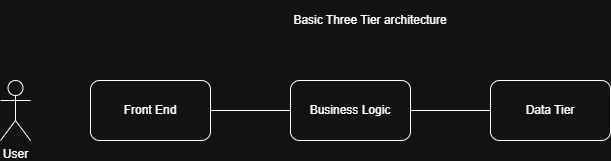
\includegraphics[width=0.8\textwidth]{basic-architecture} % Change to your filename
        \caption{Three tier architecture}
        \label{fig:drawio-diagram}
    \end{figure}


    \chapter{Architecture examples}


\end{document}
